\section{Neurons and synapses}
\label{seq:ns}

A \emph{neuron} is a cell type which occurs in all eumetazoa and therefore in most multicellular organisms. It can process and transmit electrical and chemical signals. So called \emph{synapses} are connections between neurons. Together they form neural networks. The organisms use these networks to process information.

\subsection{Structure of a typical neuron}

A typical neuron consists of:

\begin{itemize}
\item Soma (cell body): The main part of the cell, containing the organelles
\item Dendrites: Branched projection of the soma
\item Axon: Long slender projection of the soma, which has some branches in the end
\end{itemize}

\begin{figure}[!b]
	\centering
	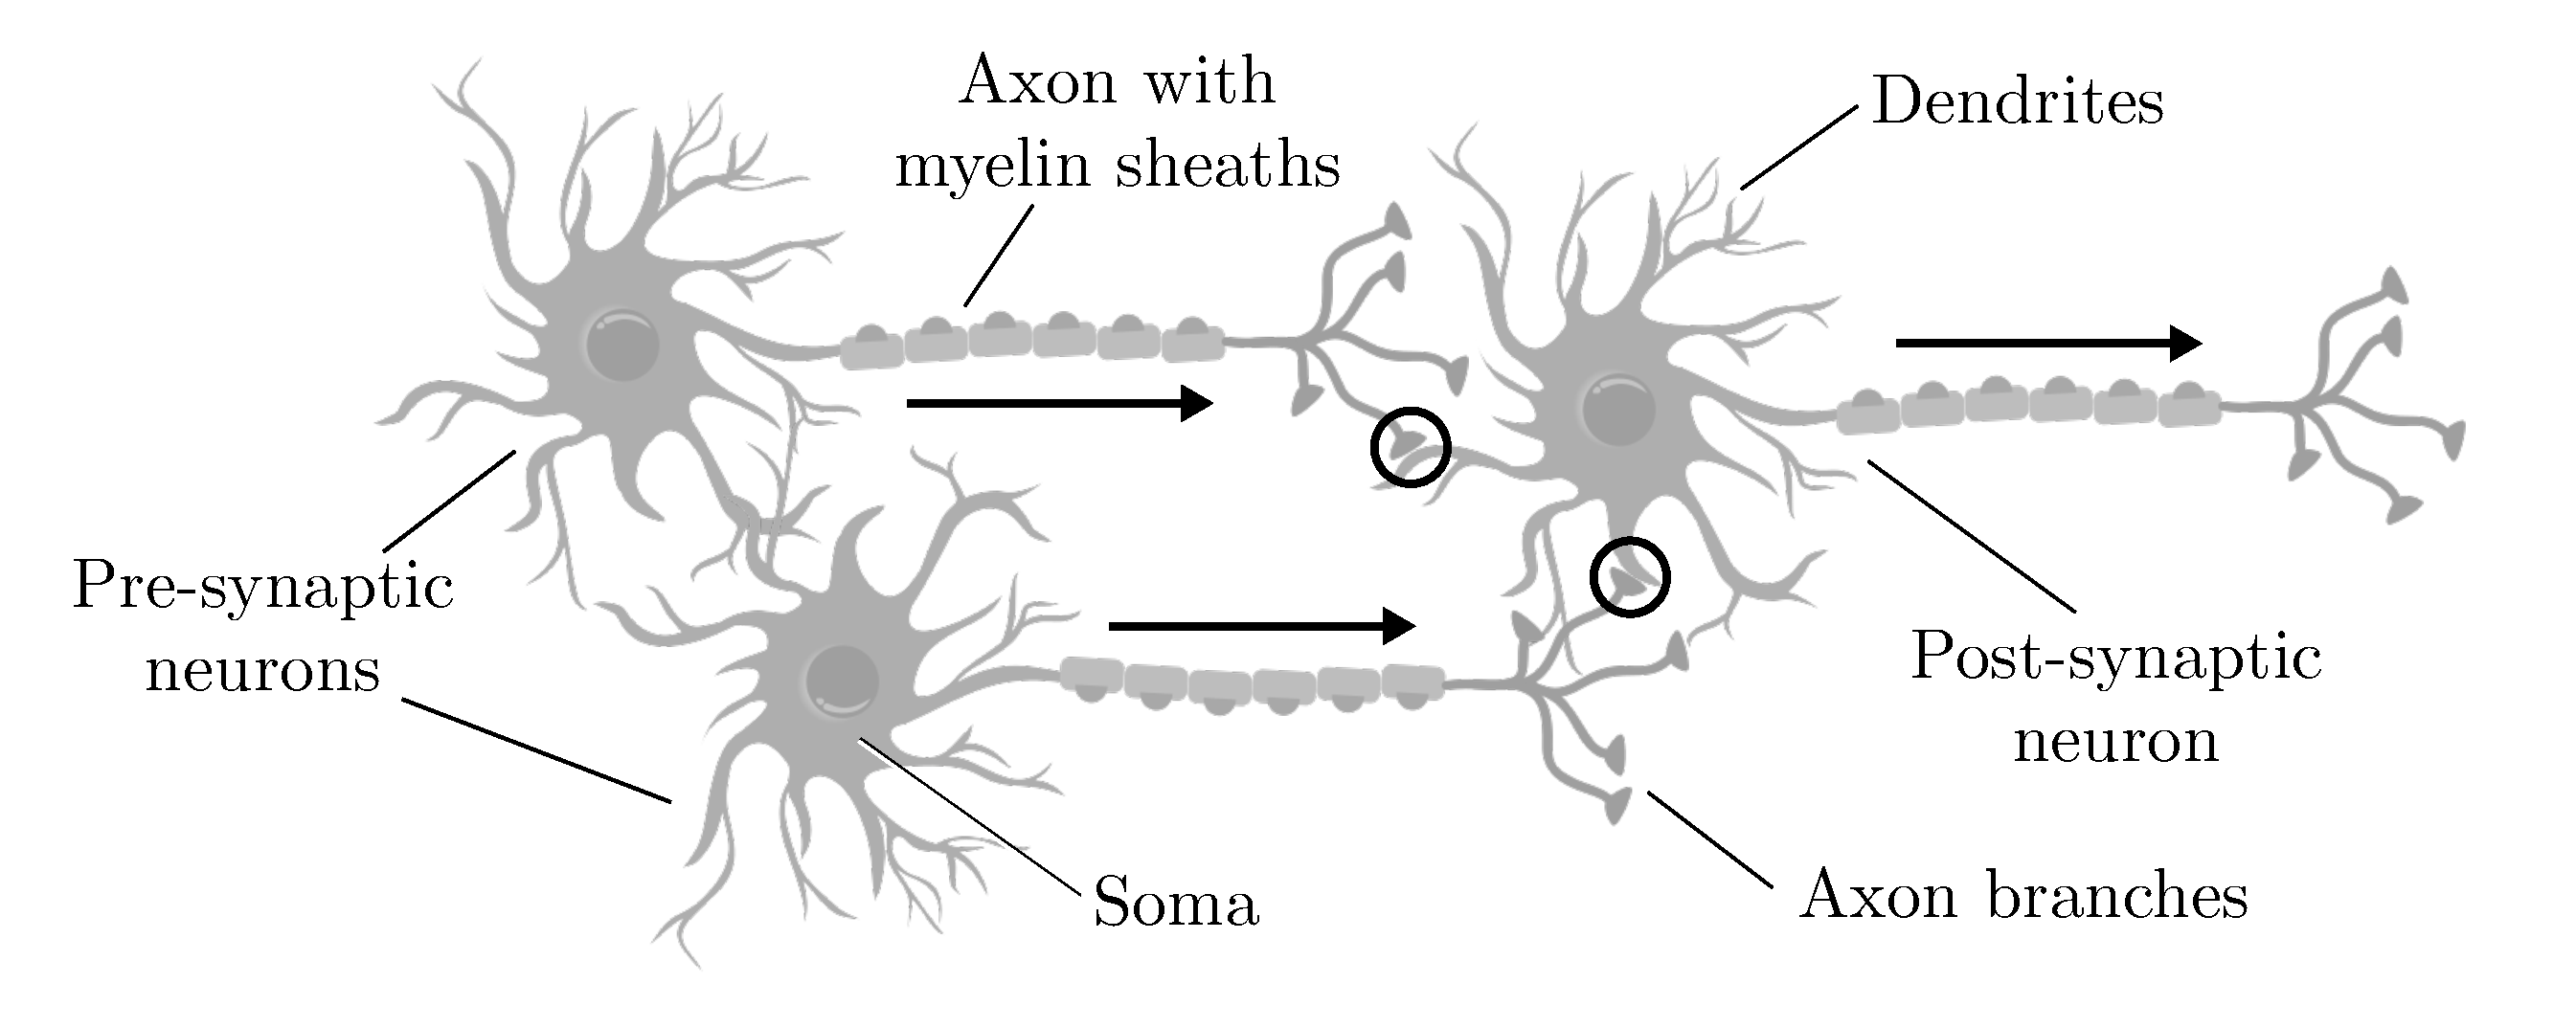
\includegraphics[width=0.8\textwidth]{neurons_plasticity/neurons}
	\caption[Structure of a typical neuron]{Three neurons showing the typical structure with soma, axon and dendrites. The synapses between presynaptic neurons and the postsynaptic neuron are highlighted with circles. The direction of the conduction is shown by arrows.\\ Adapted from: \emph{Set Of Neuron Vector.} (2017, December 16). Retrieved from https://www.vecteezy.com/vector-art/115973-set-of-neuron-vector}
	\label{fig:neurons}
\end{figure}

The dendrites and  the axon are called \emph{neurites}, which are projections from the cell body. The branches of the axon of one neuron are connected to another neurons dendrites. The connection points between the neurons are called synapses. In figure \ref{fig:neurons} a schematic representation of three neurons is shown where soma, dendrites and axon are indicated. The synapses are highlighted by circles.

\subsection{Action potential of a typical neuron}
\label{sec:act-pot}

According to \textcite{deetjen2005repetitorium}, a typical cell has a membrane potential of about $-70\,mV$ at its axon hillock, it is called the \emph{resting potential}. If the cell gets some electrical stimulation, which brings the membrane potential up to a \emph{threshold potential} of at least $-55\,mV$, the \emph{depolarisation} of the membrane potential starts, due to changes in the concentration of $Na^+$ and $K^+$ ions inside and outside of the cell. This is triggered by changes in the permeability of voltage-gated ion channels in the membrane of the neuron. The potential grows to about $40\,mV$, the \emph{action potential} or \emph{spike}. The action potential spreads over the neuron, mainly along the axon. If the axon is covered with myelin sheaths the propagation of the signal is called \emph{saltatory conduction}, which is faster than conduction without myelin sheaths.

The signals are transmitted nearly binary, where the threshold potential decides if the current activation is enough to transmit a signal or not. That principle is called \emph{all-or-none law}. The height of the threshold can vary, depending on two factors. First, directly after an activation potential was fired from the neuron, there is a short period, where the cell is not excitable at all (\emph{absolute refractory period}), which equals a threshold of infinity. After that, there is a period where the neuron is excitable again, but where the threshold is higher than normal (\emph{relative refractory period}). Both is due to ongoing recovery processes of ions in the cell. Second, the threshold is influenced by the extracellular concentration of ions, where also $Ca^{2+}$ plays an important role \parencite{deetjen2005repetitorium}.

\subsection{Structure and behavior of a typical synapse}
\label{sec:synapse}

The end of the axon or a branch of the axon of one cell (\emph{pre-synaptic cell}) is connected to the dentride of another cell (\emph{post-synaptic cell}). The cell membranes are called \emph{pre-synaptic membrane} and \emph{post-synaptic membrane} respectively. Both are shown in figure \ref{fig:synapse}.

Synapses can occur as a \emph{chemical synapse} or as an \emph{electrical synapse}. Chemical synapses transmit signals via chemical substances (\emph{neurotransmitter}), since the gap between the pre-synaptic and post-synaptic cell is $12\,nm$ to $20\,nm$ \parencite{savtchenko2007optimal} and cannot be bridged by electrical activation. The neurotransmitters need some time to reach the post-synaptic cell. Simulations show that it takes about $0.5\,ms$ until $50\%$ of the distributed transmitters receive the post-synaptic neuron, assuming a synaptic gap of $20\,nm$ \parencite{clements1996transmitter}. Electrical synapse are nearly directly connected with a gap of just $2\,nm - 3\,nm$ \parencite{peracchia1977gap}. They are connected by gap junction proteins, called \emph{connexins}, and can transmit electrical signals directly. In those synapses is nearly no delay in transmission compared to chemical synapses.

\begin{figure}[t]
	\centering
	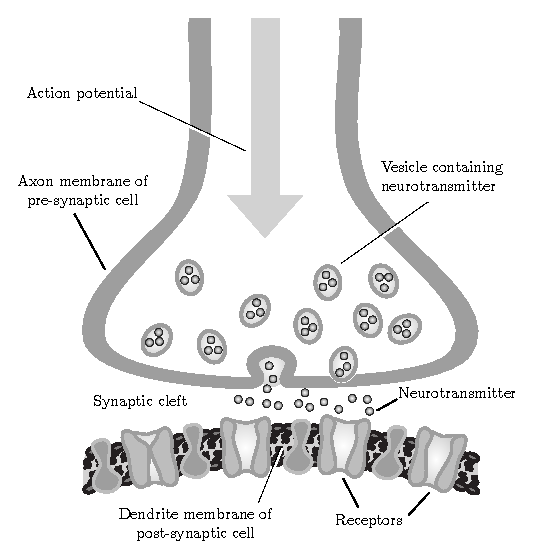
\includegraphics[width=0.6\textwidth]{neurons_plasticity/synapse}
	\caption[Structure of a typical synapse]{Structure of a typical chemical synapse. Because of an incoming potential, vesicles move to the synaptic cleft and release the containing neurotransmitter. The neurotransmitter will connect to the receptors in the membrane of the post-synaptic neuron. This causes a flow of ions in the post-synaptic membrane, changing its potential.\\ Adapted from: \textcite[p. 73]{schandry2007biologische}}
	\label{fig:synapse}
\end{figure}

In chemical synapses the pre-synaptic membrane contains the neurotransmitter, collected in \emph{vesicles}. If a potential arrives at the synapse, the vesicles move to the pre-synaptic membrane. The vesicles merge with the membrane and the neurotransmitters are released into the \emph{synaptic cleft}, the space between the pre-synaptic membrane and the post-synaptic membrane. At the post-synaptic membrane are receptors and ion channels, often they are joined to a \emph{receptor-channel-complex}. If they are combined to such a complex, the receptor is called \emph{ionotropic receptor}. The neurotransmitter binds to the ion channel and changes its structure which allows an exchange of ions. Since the neurotransmitter operates like a key which opens a lock, where the lock is the ion channel, this mechanism is called \emph{key-lock principle}. Since both parts (receptor and ion channel) are in one place, the reaction is fast \parencite[p. 40]{deetjen2005repetitorium}. In the other case, receptor and ion channels are separated and the receptor is called \emph{metabotropic receptor}. The neurotransmitter connects to a receptor, but this time the receptor releases a messenger substance called \emph{second messenger}. This second messenger finally opens an ion channel. The effect is slower, since it takes some time until the reaction inside the post-synaptic cell is ready and the ion channels are opened. A simplified scheme of a chemical synapse is shown in figure \ref{fig:synapse}.

\subsection{Inhibitory and excitatory neurons}
\label{sec:inhib-excit}

The signals, reaching the neuron via the synapses, can be \emph{inhibitory} or \emph{excitatory}. Inhibitory synapses reduce the potential and decrease the chance to reach the threshold potential that leads to an action potential. They mainly operate with GABA ($\gamma$-Aminobutyric acid), Glycine, Serotonin or Dopamin as neurotransmitter. Excitatory synapses rise the potential and therefore increase the chance to start an action potential. They mainly use Acetylcholine or Noradrenalin. Both types of synapses have different chemical mechanisms to change the potential. According to \emph{Dale's principle}, a neuron has either only inhibitory or excitatory axonal synapses \parencite{dale1935pharmacology, eccles1976electrical}. There are exceptions from this rule, but in most cases the principle holds \parencite{sossin1990dale}. If a neuron has inhibitory outgoing synapses, it is called an \emph{inhibitory neuron}. In case of excitatory synapses it is called \emph{excitatory neuron}.

The incoming signals from all connected synapses --- which can be several thousands \parencite[p. 89]{schandry2007biologische} --- sum up to an overall potential at the soma of the post-synaptic neuron. The summation can be spatial or temporal. \emph{Spatial summation} means that the potential is rising if many different synapses are active at the same time. \emph{Temporal summation} describes a process where at a synapse many signals are coming in a row and sum up to a higher overall potential. The time gap between the signals can be very different, depending on the type of synapse. In some synapse it is necessary, that the signals must be closer than $20\,ms$ to each other to have a summing effect, in some synapses a gap of $1\,s$ can still influence the potential \parencite[p. 92]{schandry2007biologische}.

In many artificial networks the neuron $i$ is modeled with a specific activation $a_i$ at a time, which is linearly dependent from incoming signals. In that case spatial summation can be modeled with

\begin{equation}
\label{eq:activation}
a_i = \sum_{j=1}^{n_i} w_{ij} z_{j} - t_i,
\end{equation}

where $n_i$ is the number of potential input signals (number of synapses), $z_{j}$ the activation of the single sources and $w_{ij}$ the weights from the pre-synaptic neuron to the post-synaptic neuron. $t_i$ is the threshold of the post-synaptic neuron.

The transmission of a signal from one neuron to another is modeled with an \emph{activation function} $\sigma(a_i)$ that modulates the intensity and can decide if the neuron is sending a signal or not. To model the binary output of a biological network an indicator function can be used, like the \emph{Heaviside step function}

\nomenclature{$\sigma(a_i)$}{Activation function}

\begin{equation}
\label{eq:heavi}
\sigma(a_i) = \Theta(a_i) = \begin{cases}
\;0, & a_i < 0\\
\;1, & a_i \ge 0
\end{cases}.
\end{equation}

If the activation $\sum_{j=1}^{n_i} w_{ij} z_{j}$, coming from the pre-synaptic neurons, is higher than the threshold $t_i$, the Heaviside function is equal to one and an action potential of the post-synaptic neuron is simulated.

In many cases it is necessary to calculate derivations of the activation function (e.g. for the backpropagation algorithm, which is widely used in machine learning). In that case smooth approximations like the sigmoid function can be used. Statistically the activation function $\sigma$ is the inverse of the link function in a \acfi{glm} and therefore the part that brings non-linearity to the model, since $a_i$ is a linear function. In case of the sigmoid function, the activation function at every neuron is equal to a logistic regression. Further details regarding the mathematical model are given in section \ref{sec:ann}.

\subsection{Classifications of neurons}

In general, neurons can be classified by their function \parencite[p. 39]{schandry2007biologische}.

\begin{itemize}
\item \emph{Sensory neurons}: Receives information from a sensory cell
\item \emph{Motor neurons}: The axon is connected to a muscle
\item \emph{Interneurons}: The most common type, which receives from and sends information to other neurons
\end{itemize}

In artificial neural networks the \emph{input} can be seen as sensory neurons in living beings, where the whole network structure is equivalent to the interneurons. The \emph{readout} of a network is analog to the current state of the interneurons. The \emph{output} is similar to the motor neurons which could, for instance in robotics, control some electric motors.

Neurons can also be classified morphologically.

\begin{enumerate}
\item \emph{Unipolar neuron}: Has just one neurite, mostly one axon
\item \emph{Bipolar neuron}: Has two neurites, one axon and one dendrite
\item \emph{Multipolar neuron}: Has many neurites, one axon and many dendrites
\item \emph{Anaxonic neuron}: Axon and dendrites cannot be differentiated
\end{enumerate}

\begin{wrapfigure}{r}{0.45\textwidth}
	\centering
	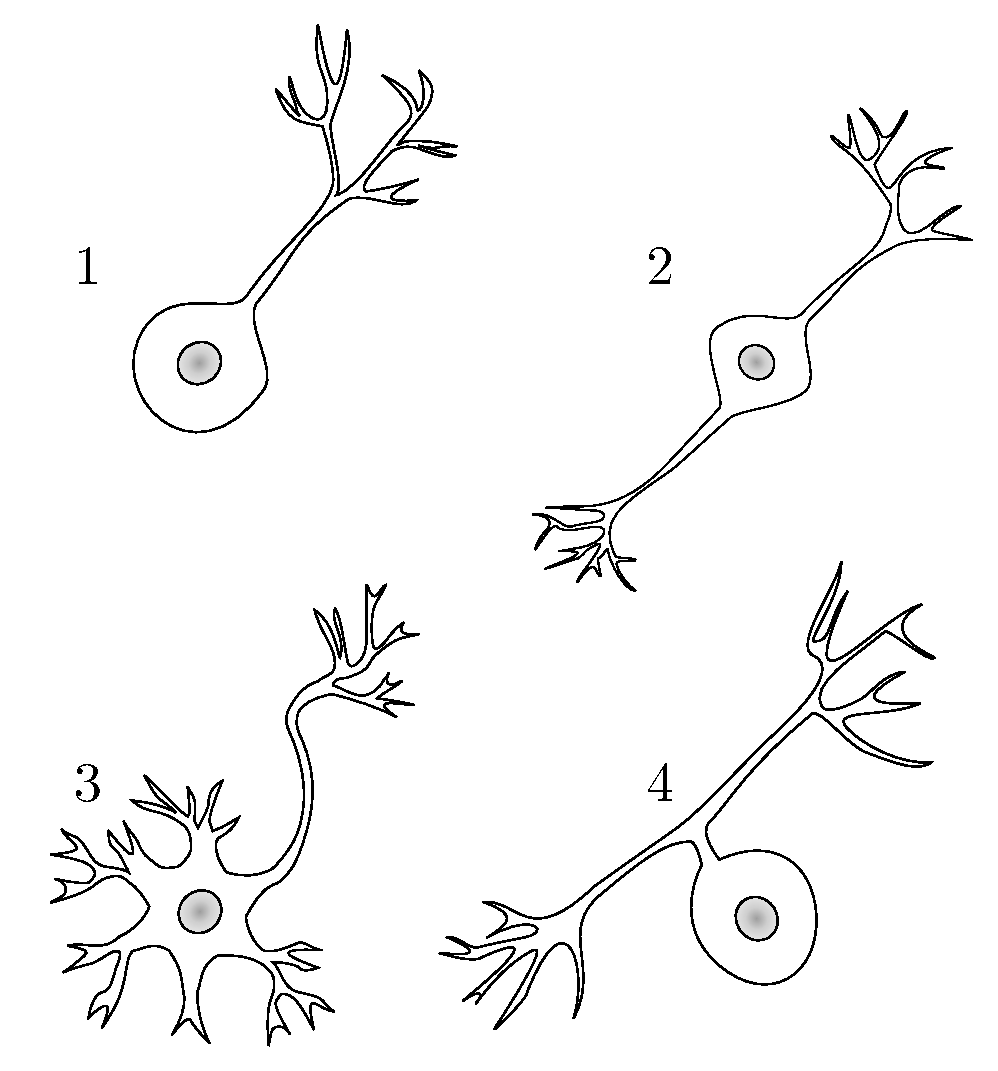
\includegraphics[width=0.45\textwidth]{neurons_plasticity/neuron_types}
	\caption[Morphological classification of neurons]{Morphological classification of neurons: (1) Unipolar neuron, (2) Bipolar neuron, (3) Multipolar neuron and (4) Anaxonic neuron.\\ Adapted from: \emph{Neuron.} (2017, December 16). Retrieved from https://en.wikipedia.org/wiki/Neuron}
    \vspace{10pt}
    \label{sec:neuron-types}
\end{wrapfigure}

All four types are are shown in figure \ref{sec:neuron-types}. There are many specialized cells like for example purkinje cells, which are large multiplolar interneurons in cerebellum, or pyramidal cells, which are multipolar interneurons in many areas of the brain. Pyramidal cells, for example, are the main source for measurements using electroencephalography \parencite{kirschstein2009source}.

In many artificial networks, like the one which is used in this thesis, the input is designed with a neuron which has just an axon with some projections, the output has just dendrites. Inbetween are multipolar or rarely bipolar neurons, which form the characterizing part of the artificial neural network. As well as in the brains of living beings, the most common neuron in artificial neural networks is modeled with the multipolar neuron.
